\chapter{Conceptual Model}

Figure \ref{fig:mockup} below outlines a conceptual model of the web interface for our system.

\begin{figure}[h]
	\centering
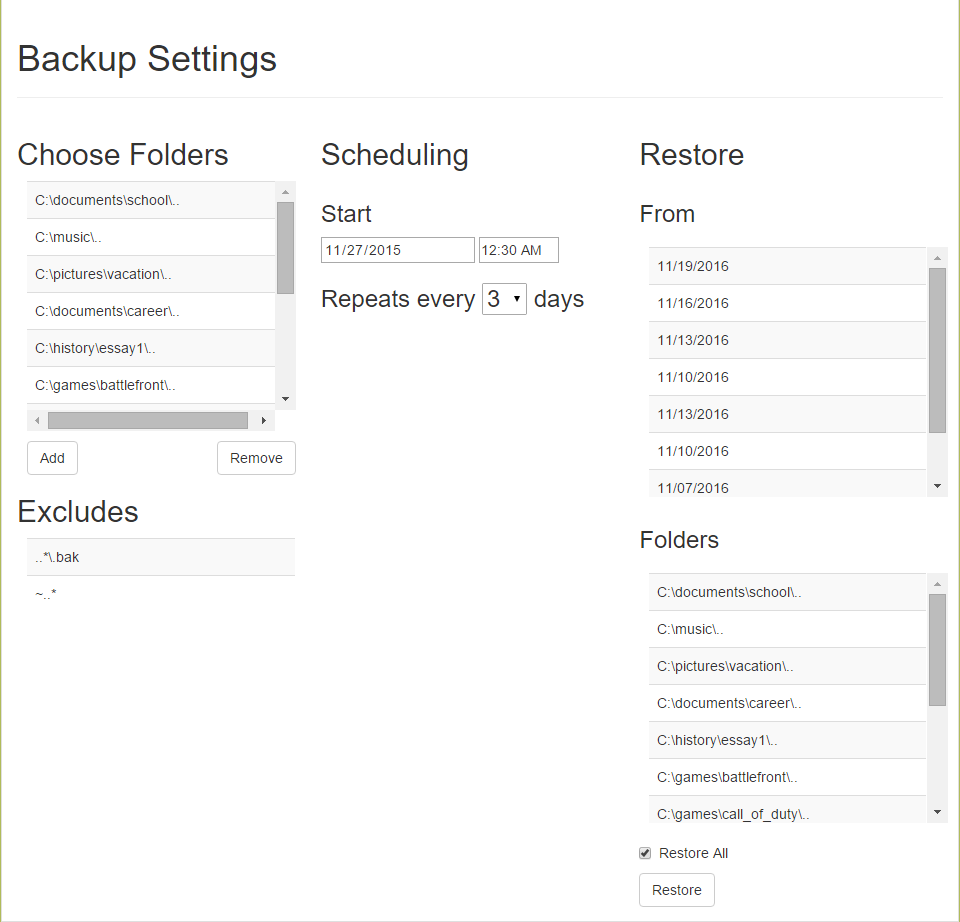
\includegraphics[scale=0.45]{images/mockup.png}
	\caption{Web Interface Conceptual Model}
	\label{fig:mockup}
\end{figure}

\chapter{Activity Diagram}

Our activity digram (figure \ref{fig:activitydiagram} below) is pretty straightforward.  An end user will interact with our system mainly through the web interface.  This interface displays all of the controls on a single page, so most settings can be altered in a single step.  For example, adding or removing folders to be backed up can be done in a single step, as can be setting backup times.  The only somewhat complex activity is that of restoring folders.  First the user should choose the restore point in order to get a list of what folders are available from that point in time.  Then the user either selects specific folders or all of them to restore.  When the user is done changing settings, they can simply leave.

\begin{figure}[h]
	\centering

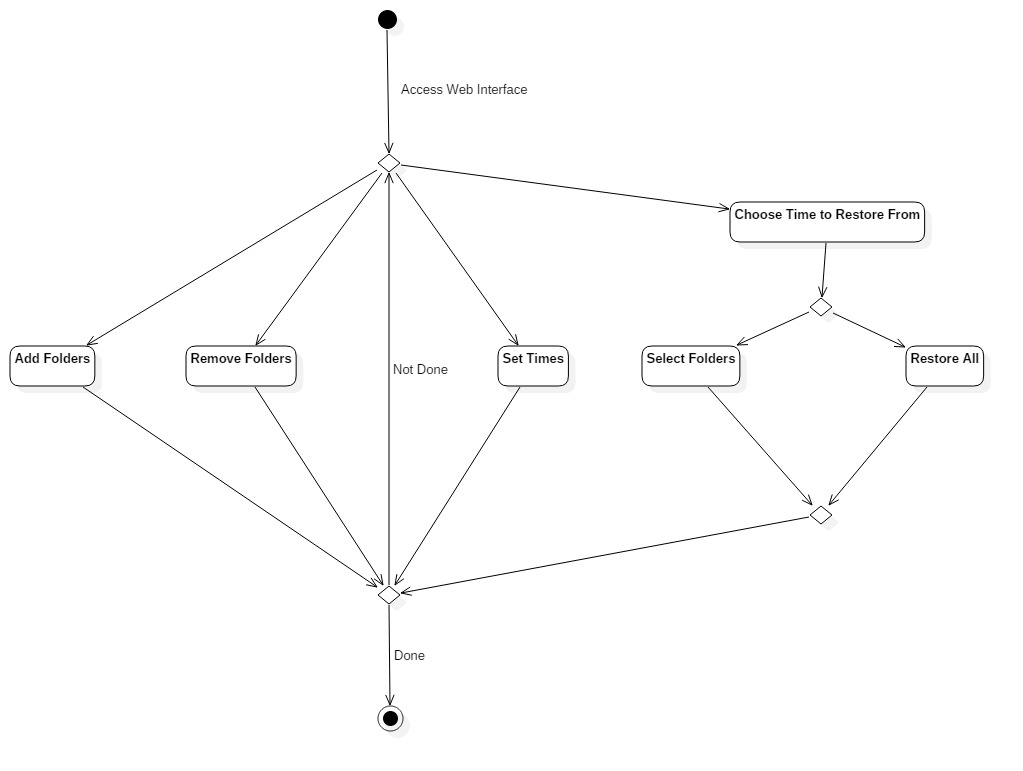
\includegraphics[scale=0.45]{images/ActivityDiagram1.jpg}
	\caption{Web Interface Activity Diagram}
	\label{fig:activitydiagram}
\end{figure}